\documentclass{article}

% FONTS
\usepackage[T1]{fontenc}

\usepackage{tgtermes}
\usepackage{amsmath}
\usepackage{amssymb}
%\usepackage[subscriptcorrection,
%            amssymbols,
%            mtpbb,
%            mtpcal,
%            nofontinfo  % suppresses all warnings
%           ]{mtpro2}
\usepackage{scalefnt,letltxmacro}
\LetLtxMacro{\oldtextsc}{\textsc}
\renewcommand{\textsc}[1]{\oldtextsc{\scalefont{1.10}#1}}
\usepackage[scaled=0.92]{PTSans}
\usepackage{inconsolata}

% COLOR
\usepackage[usenames,dvipsnames]{xcolor}
\definecolor{shadecolor}{gray}{0.9}

% SPACING and TEXT
\usepackage[final, expansion=alltext]{microtype}
\usepackage[english]{babel}
\usepackage{afterpage}
\usepackage{framed}
\usepackage{nicefrac}

% Define a paragraph header function
\DeclareRobustCommand{\parhead}[1]{\textbf{#1}~}

% paragraph helper
\DeclareRobustCommand{\PP}{\textcolor{Plum}{\texttt{\P}}~}
\DeclareRobustCommand{\pp}{\textcolor{Plum}{\texttt{\P}}~}

% COUNTERS
\renewcommand{\labelenumi}{\color{black!67}{\arabic{enumi}.}}
\renewcommand{\labelenumii}{{\color{black!67}(\alph{enumii})}}
\renewcommand{\labelitemi}{{\color{black!67}\textbullet}}

% FIGURES
\usepackage{graphicx}
\usepackage[labelfont=bf]{caption}
\usepackage[format=hang]{subcaption}

% TABLES
\usepackage{booktabs}

% BIBLIOGRAPHY
\usepackage{natbib}

% ALGORITHMS
\usepackage[algoruled]{algorithm2e}
\usepackage{listings}
\usepackage{fancyvrb}
\fvset{fontsize=\normalsize}

% HYPERREF
\usepackage[colorlinks, linktoc=all]{hyperref}
\usepackage[all]{hypcap}
\hypersetup{citecolor=Violet}
\hypersetup{linkcolor=black}
\hypersetup{urlcolor=MidnightBlue}

% CLEVEREF must come after HYPERREF
\usepackage[nameinlink]{cleveref}

% ACRONYMS
\usepackage[acronym,smallcaps,nowarn]{glossaries}
% \makeglossaries

% COLOR DEFINITIONS
\newcommand{\red}[1]{\textcolor{BrickRed}{#1}}
\newcommand{\orange}[1]{\textcolor{BurntOrange}{#1}}
\newcommand{\green}[1]{\textcolor{OliveGreen}{#1}}
\newcommand{\blue}[1]{\textcolor{MidnightBlue}{#1}}
\newcommand{\gray}[1]{\textcolor{black!60}{#1}}

% LISTINGS DEFINTIONS
\usepackage{listings}
\lstdefinestyle{mystyle}{
    commentstyle=\color{OliveGreen},
    numberstyle=\tiny\color{black!60},
    stringstyle=\color{BrickRed},
    basicstyle=\ttfamily\scriptsize,
    breakatwhitespace=false,
    breaklines=true,
    captionpos=b,
    keepspaces=true,
    numbers=none,
    numbersep=5pt,
    showspaces=false,
    showstringspaces=false,
    showtabs=false,
    tabsize=2
}
\lstset{style=mystyle}

\input{preamble/preamble_math.tex}
% !TEX root = template.tex

\newacronym{KL}{kl}{Kullback-Leibler}
\newacronym{ELBO}{elbo}{evidence lower bound}
\newacronym{SVI}{svi}{stochastic variational inference}
\newacronym{GMM}{gmm}{Gaussian mixture model}
\newacronym{LDA}{lda}{latent Dirichlet allocation}



\usepackage{blindtext}

\usepackage{nips_2017}
\title{Reparameterizing the Birkhoff Polytope for \\ Variational Permutation Inference}


\author{
  Great Author 1 \\
  \And
  Great Author 2 \\
  \And
  Great Author 3 \\
  \And
  Great Author 4 \\
  \And
  Great Author 5 \\
}


\begin{document}

\maketitle

\begin{abstract}
  How to perform posterior inference over the space of permutation
  matrices?  By definition, with~$n$ nodes, there are~$n!$ such
  matrices.  Clearly, estimating a complete probability mass function
  over this space quicky becomes intractable as~$n$ grows. Our goal is
  to derive a tractable algorithm for performing approximate inference
  over this challenging discrete space.  To that end, we consider
  extensions of the recently proposed Gumbel-softmax method, which
  leverages continuous relaxations to perform discrete variational
  inference with reparameterization gradients. While the
  Gumbel-softmax method is not immediately applicable to permutation
  inference, we show that two alternative reparameterizations are both
  comparable to Gumbel-softmax on tractable discrete problems and
  easily extensible to permutation inference. Specifically, we develop
  continuous relaxations of permutation matrices to matrices that are
  either exactly or nearly doubly stochastic, i.e. to points either in
  or near the Birkhoff polytope.  We then derive invertible and
  differentiable maps from densities on unconstrained space to
  densities on or near the Birkhoff polytope. These transformations
  are parameterized by a ``temperature'' that controls how
  concentrated the resulting density is at the extrema of the Birkhoff
  polytope; i.e. at permutation matrices.  This relaxation admits
  variational inference via stochastic gradient ascent over the
  distributions on doubly stochastic matrices (and in the
  zero-temperature limit, on permutation matrices) using Monte Carlo
  estimates of the reparameterized gradient.
\end{abstract}

\section{Introduction}

% Permutation inference central to many machine learning problems
% - Matching problems
% - Multiple object tracking
% - Ranking
% - As latent step in a generative model
Permutation inference is central to many modern machine learning
problems.  Identity management~\citep{guibas2008identity} and
multiple-object tracking~\citep{shin2005lazy, kondor2007multi} are
fundamentally concerned with finding a permutation that maps an
observed set of items to a set of canonical labels.
Ranking problems, critical to search and recommender systems, require
inference over the space of item orderings \citep{meilua2007consensus,
  lebanon2008non, adams2011ranking}.  Moreover, many probabilistic models, like
preferential attachment network models~\citep{bloem2016random} and
repulsive point process models~\citep{rao2016bayesian}, incorporate a
latent permutation into their generative processes; inference over
model parameters requires integrating over the set of permutations
that could have given rise to the observed data.  In many of these
settings, permutation inference is but one component of a larger
estimation problem involving unknown model parameters and hierarchical
structure.

% Emphasize the importance of Bayesian approach and recent advances
% in variational inference 
While the problem of finding optimal point estimates of permutations
under a variety of cost functions has been the subject of decades of
research in combinatorial optimization\todo{cite}, many probabilistic
tasks require reasoning over uncertainty regarding permutation
matrices.  Many works have addressed the challenge of Bayesian
permutation inference, leveraging Markov chain Monte Carlo methods
\citep{diaconis1988group}, Fourier
representations~\citep{kondor2007multi, huang2009fourier}, as well as
convex~\citep{lim2014beyond} and
continuous~\citep{plis2011directional} relaxations for approximating
the posterior distribution.  Given recent advances in scaling variational
Bayesian inference, largely driven by efficient Monte Carlo estimators
of gradients of the variational lower bound \citep{Kingma2014, rezende2014stochastic},
we revisit the problem of permutation inference from a variational perspective. 


% Gumbel-softmax motivation
Motivated by the recently proposed Gumbel-softmax method for discrete
variational inference~\citep{jang2016categorical,
  maddison2016concrete}, we consider a variety of continuous
relaxations of permutations that enable gradient-based inference.  The
Gumbel-softmax method is based on the following observation: discrete
distributions may be viewed as atomic densities on the vertices of the
simplex; by relaxing this to a continuous density on the interior of
the simplex we can approximate the discrete inference problem with a
continuous one and thereby capitalize on reparameterization
gradients~\citep{Kingma2014, rezende2014stochastic} to optimize a
variational lower bound on the marginal likelihood.  Critically, the
Gumbel-softmax method has a temperature parameter that tunes the
degree to which the continuous density concentrates around the
vertices, and recovers truly discrete inference in the
zero-temperature limit.

% Discrete/Simplex <-> Permutation/Birkhoff analogy 
Just as one-hot vectors (discrete random variables) are the vertices
of the simplex, permutation matrices are the vertices of the Birkhoff
polytope, i.e. the set of doubly stochastic matrices.  Analogously to
the Gumbel-softmax method, we seek temperature-controlled relaxations
of atomic densities on permutation matrices to continuous densities on
the interior of the Birkhoff polytope.  Unfortunately, due to the
dual constraints of row- and column-normalization required of doubly
stochastic matrices, the Gumbel-softmax method does not immmediately
extend to this more challenging domain.  However, we derive a variety
of alternative continuous relaxations for the simplex and show that:
(i) these relaxations achieve comparable performance to the Gumbel-softmax
  on tractable discrete inference tasks; and
(ii) they naturally extend to relaxations of permutation inference
  problems. 

% Paper structure
The remainder of this paper is structured as follows: Section~\ref{sec:relatedwork}
discusses related work on Bayesian permutation inference, and Section~\ref{sec:gumbel}
introduces the Gumbel-softmax relaxation upon which our approach builds.
Section~\ref{sec:alternative} introduces alternative relaxations for
discrete variational inference, and Section~\ref{sec:permutation} presents
our primary contribution: a set of relaxations for permutation matrices
Sections~\ref{sec:synthetic}-\ref{sec:synth_celegans} detail a variety
of experiments that illustrate the value of our variational approach.
  
\section{Related Work}
\label{sec:relatedwork}

\begin{itemize}
  \item MCMC \citep{diaconis1988group} methods are successful
in some cases, but ultimately rely on local updates to randomly
explore the high dimensional space of permutations.

  \item Fourier \citep{kondor2007multi, huang2009fourier}

  \item Convex relaxations? \citep{lim2014beyond}

  \item Other continuous relaxations \citep{plis2011directional}
\end{itemize}

\section{The Gumbel-softmax relaxation for discrete variational inference}
\label{sec:gumbel}

In Bayesian inference problems, we have a prior distribution~$p(x)$
and a likelihood~$p(y \mid x)$, and
we seek the posterior distribution,~${p(x \mid y) = p(x) p(y \mid x) / p(y)}$.
%The output a distribution over vertices of the simplex.
In general, this problem is intractable since the normalizing constant
in Bayes' rule, $p(y)$, involves a high dimensional integral or sum.
Variational inference algorithms avoid this problem by limiting their
search to a tractable family of distributions,~$q(x; \theta)$,
parameterized by~$\theta$, and searching for the member of this family
that best approximates the true posterior. Most commonly, the
approximation quality is measured by the Kullback-Leibler (KL)
divergence between the variational posterior,~$q(x; \theta)$, and the
true posterior,~$p(x \mid y)$. That is, the optimal variational
parameters are given by,
\begin{align}
  \theta^* &= \argmax_\theta -\KL{q(x; \theta)}{p(x \mid y)},
\end{align}
where
\begin{align}
  -\KL{q(x; \theta)}{p(x \mid y)} 
  &= \E_{q}
  \left[ \log p(x \mid y) - \log q(x; \theta) \right] \\
  &\geq \E_{q}
  \left[ \log p(x, \, y) - \log q(x; \theta) \right] \\
  &= \cL(\theta).
\end{align}
The objective function,~$\cL(\theta)$, is known as the evidence lower bound, or ELBO.
Stochastic gradient ascent is
perhaps the simplest method of optimizing the ELBO with respect to
the parameters~$\theta$.
However, computing~$\nabla_\theta \cL(\theta)$ requires some care,
since the ELBO contains an expectation with respect to a distribution
that depends on these parameters.

When~$x$ is a continuous random variable, we can often go one step
further and leverage the ``reparameterization trick''  \citep{Salimans2013,Kingma2014,Price1958,Bonnet1964}.  Specifically,
in some cases we can simulate from~$q$ via the following procedure,
\begin{align}
\xi &\sim p(\xi),  \\
x &= g(\theta, \xi),
\end{align}
where~$g(\theta, \xi)$ is a deterministic and differentiable
transformation (which is only possible if~$x$ is continuous). Thus, we
can effectively ``factor out'' the randomness of~$q$. With this
transformation, we can bring the gradient inside the expectation as
follows,
\begin{align}
%  \nabla_\theta \E_{q(x \mid \theta)} \left[ \log p(x \mid y) - \log q(x; \theta) \right]
  \nabla_\theta \cL(\theta) 
  &= \E_{p(\xi)} \left[ \nabla_\theta \left[\log p(g(\theta, \xi) \mid y) - \log q(g(\theta, \xi); \theta) \right] \right].
  %\\
%  &\approx \frac{1}{M} \sum_{m=1}^M \nabla_\theta \log p(g(\theta, \xi^{(m)}) \mid y) - \log q(g(\theta, \xi^{(m)}); \theta) & & & \xi^{(m)} &\sim p(\xi).
\end{align}
This gradient can be estimated with Monte Carlo, and, in practice,
this leads to lower variance estimates of the gradient than, for
example, the score function estimator \citep{Williams1992,Glynn1990}.

\begin{figure*}[t]
  \centering
  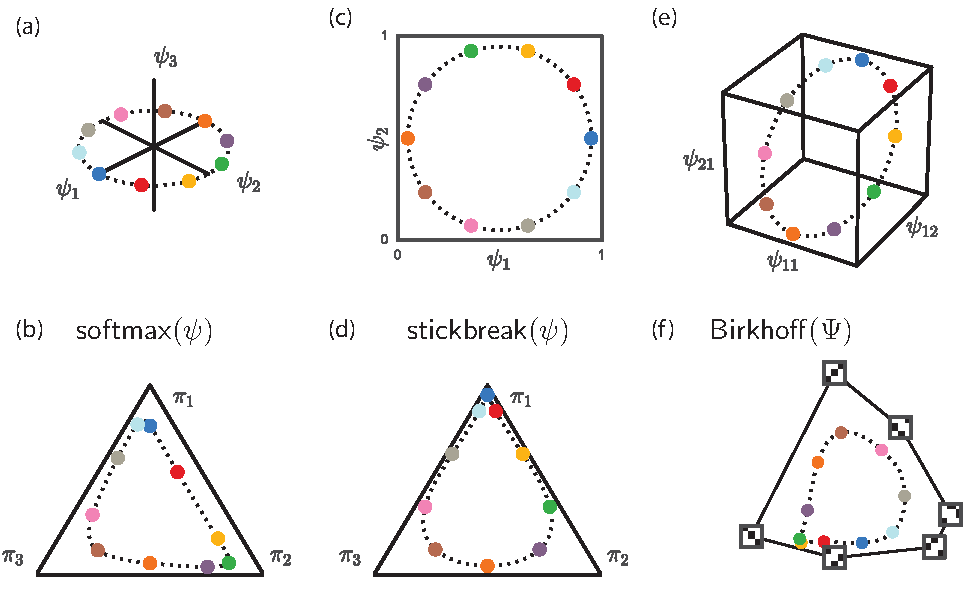
\includegraphics[width=5.in]{../figures/figure1.pdf} 
  \caption{
  }
\label{fig:transforms}
\end{figure*}



Recently, there have been a number of proposals for extending these
reparameterization tricks to high dimensional discrete
problems\footnote{Discrete inference is only problematic in the high
dimensional case, since in low dimensional problems we can enumerate
the possible values of~$x$ and compute the normalizing constant~$p(y)
= \sum_x p(y, x)$.} by relaxing them to analogous continuous
problems \citep{maddison2016concrete, jang2016categorical,
kusner2016gans}.  These approaches are based on the following
observation: if~$x \in \{0,1\}^k$ is a one-hot vector drawn from a
categorical distribution, then the support of~$p(x)$ is the set of
vertices of the~$k-1$ dimensional simplex.  Thus, we can represent the
distribution of~$x$ as an atomic density on the simplex.  Sampling~$x$
is equivalent to sampling this atomic measure. That is,
\begin{align}
  x &\sim \distCategorical( x \mid \theta) &\iff& & {\pi} &\sim p({\pi} \mid \theta) \nonumber \\
  & & & & x &\triangleq {\pi},
\end{align}
where~$p({\pi} \mid \theta)$ is a density on the simplex with atoms at
the~$k$ vertices.

Viewing~$x$ as a vertex of the simplex motivates a natural relaxation:
let us set~$x={\pi}$ as above, but 
rather than restricting~$p({\pi} \mid \theta)$ to be an atomic measure,
let it be a continuous density on the simplex. To be concrete, suppose
the density of~${\pi}$ is defined by the transformation,
\begin{align}
  \xi &\sim p(\xi), \\
  {\pi} &= g(\theta, \xi) \\
  g(\theta, \xi) &= \text{softmax}(\log \theta + \xi).
\end{align}
The output~$x$ is now a point on the simplex, and the parameters~$\theta$ can
be optimized via stochastic gradient ascent with the reparameterization trick,
as discussed above.

In the aforementioned papers,~$p(\xi)$ is taken to be the Gumbel distribution.
This choice leads to a nicely interpretable model: adding
Gumbel noise and taking the argmax yields an exact sample from~$\theta$;
setting~$g$ to the softmax is a natural relaxation. Ultimately, however, this
is just a continuous relaxation of an atomic density to a continuous
density. 

\section{Alternative continuous relaxations}
\label{sec:alternative}

While the Gumbel-softmax has some nice properties, as we will see, it does
not lend itself as naturally to more complicated generalizations. 
Consider the following alternative model for~${\pi}$:
\begin{align}
  \psi_k &\sim \distNormal(\mu_k, \tau^{-1} \eta_k^2) & &  \text{for } k=1, \ldots, K-1\\
  {\pi}_1 &= \sigma(\psi_1) \\
%  {\pi}_k &= \sigma(\psi_k) \prod_{j=1}^{k-1} (1-\sigma(\psi_j)) & &  \text{for } k=2, \ldots, K-1\\
  {\pi}_k &= \sigma(\psi_k) (1- \sum_{j=1}^{k-1} {\pi}_j) & &  \text{for } k=2, \ldots, K-1\\
%  {\pi}_K &= \prod_{j=1}^{K-1} (1-\sigma(\psi_j))
{\pi}_K &= 1- \sum_{j=1}^{K-1} {\pi}_j
\end{align}
This is known as a logistic stick breaking transformation since
~$\sigma(\cdot)$ is the logistic function and~$\sigma(\psi_k)$ can be
seen as the fraction of the remaining ``stick'' of probability mass
assigned to~${\pi}_k$ \citep{linderman2015dependent}. Moreover,
the density of~${\pi}$ can be expressed in closed form as a
function of~$\mu_k$ and~$\eta_k^2$.  Finally, as with the relaxations
above, the temperature~$\tau$ controls how
concentrated~$p_\tau({\pi} \mid \{\mu_k, \eta_k^2\})$ is at the
vertices of the simplex. As~$\tau \to 0$, the density becomes
concentrated on atoms at the~$K$ vertices, and as~$\tau \to \infty$,
the density concentrates on a point in the interior of the simplex
determined by~$\{\mu_k\}$. For intermediate values, the density is
continuous on the simplex.

\subsection{Limit analysis}
\todo{appendix}
One nice property of the concrete distribution \citep{maddison2016concrete, jang2016categorical} is that it can be understood as the 'heating' of the original categorical distribution (equivalently, a probability simplex-valued distribution whose atoms are the vertices of the simplex): specifically, in the high temperature limit ($\tau \rightarrow \infty$) the distribution becomes a single atom in the center of mass of the probability simplex, while the zero-temperature limit ($\tau\rightarrow 0$) corresponds to the target categorical distribution. Now we show that although the stick-breaking representation may seem 'position biased', in reality, through appropriate choices of the parameters we are able to provide richer representations as compared to the concrete case. Specifically, we will show that degenerate cases can correspond to arbitrary categorical distributions and arbitrary point masses in the simplex.

To see this, consider first the more general stick-breaking representation
\begin{align}
  \psi_k & = g(\theta_k,\epsilon_k)& &  \text{for } k=1, \ldots, K-1\\
  {\pi}_1 &= \psi_1 \\
  {\pi}_k &= \psi_k \left(1- \sum_{j=1}^{k-1} {\pi}_j\right) & &  \text{for } k=2, \ldots, K-1\\
%  {\pi}_K &= \prod_{j=1}^{K-1} (1-\sigma(\psi_j))
{\pi}_K &= 1- \sum_{j=1}^{K-1} {\pi}_j.
\end{align}

Where $g$ is a $[0,1]$-valued function. 

The following lemmas analyze two degenerate but useful cases:

\textbf{Proposition:}  the degenerate case where $\psi_k=g(\theta_k)$ (i.e, $\psi_k$ is non-random) leads to $\pi\sim \delta(\tilde{\pi})$  (i.e, single atom in the point $\tilde{\pi}$) with $\pi$ in $\Delta^{k-1}$ is computed from the above formulae. Also, if any point in $[0,1]$ can be realized through $g(\theta_k)$ then any deterministic $\pi$ can be realized.

\textit{Proof}: The first part is obvious. The second part is also obvious, once acknowledging the invertibility of the function $f$ that maps $\psi \xrightarrow{f} \pi$.

\textbf{Proposition:} the degenerate case where  $\psi_k$ are Bernoulli with some parameter $p_{\theta_k}$) leads to $\pi$ having an atomic distribution with atoms in the vertices of $\Delta^{k-1}$ (i.e, $\pi$ is categorical). We have the following expression for the probabilities of the atoms $\pi_k=1$ (one hot vectors):
\begin{align}
P(\pi_k =1)&= \prod_{i=1}^{k-1} (1-p_{\theta_i}) p_{\theta_k}  & &\text{for } k=1, \ldots, K-1,\\
P(\pi_K =1) &= \prod_{i=1}^{K-1} (1-p_{\theta_i}).
\end{align}
Moreover, if any Bernoulli variable can be realized through appropriate choice of the parameters then, any categorical distribution can be realized.
\textit{Proof}: the first expression comes from expressing the event $\pi_k=1$ equivalently as $\pi_k=1,p_i=0 i<k$ and then, conditioning backwards successively. The second comes from the following (which is deduced by replacing terms in the above)
$$ p_{\theta_k}=\frac{P(\pi_k =1)}{P(\pi_{k-1} =1)}\frac{p_{\theta_{k-1}}}{1-p_{\theta_{k-1}}},\quad k =1,\ldots, K-1.$$
The recursive nature of the above equation gives a recipe to iteratively determine the required $p_{\theta_k}$, given  $P(\pi_k =1), P(\pi_{k-1} =1)$ and the already computed $p_{\theta_{k-1}}$.

Having stated the above properties it only remains showing that the two re-parameterizations we consider here, based on the Gaussian and Kumaraswamy distributions, lead to the above degenerate distribution as their limits.

\textbf{Proposition} For the choice $\psi=\sigma(\delta),\delta\sim\mathcal{N}(\mu,\eta^2)$, the limit $\eta\rightarrow 0$ leads to the non-random $\psi=\sigma(\mu)$. Additionally, the limit $\mu\rightarrow \infty, \eta^2=\mu/K$ with K constant leads to $\psi\sim \text{Bernoulli}(\Phi(K))$ ($\Phi$ denotes the standard normal cdf). In both cases the convergence is in distribution \textit{Proof}. The first convergence is obvious. To see the second, let's index $\mu_n$ and  study the cdf of $\Psi_n$ and 
\begin{align}F_{\Psi_n}(x)&=& P(\sigma(\delta_n)<x) \\
&=&P(\delta_n< \sigma^{-1}(x))\\
&=& P(\mu_n +\mu_n/K\epsilon <\sigma^{-1}(x)),\\\
&=& P( \epsilon <\sigma^{-1}(x))K/\mu_n -K)\\
&=& \Phi( \sigma^{-1}(x))K/\mu_n -K) 
\end{align}
Therefore, by continuity of $\Phi$ we obtain $F_{\Psi_n}(x)\rightarrow \Phi(-K)$ for all points $x\in(,1)$. On the other hand, the cdf of a bernoulli random $F$ variable is given by  a step function that abruptly changes at zero from (zero to $1-p$), and at one (from $1-p$ to 1. As we have obtained convergence to $F$ at all ints continuity points (the interval $(0,1)$), with $1-p= \Phi(-K)\rightarrow \Phi(K)=p$) so we can conclude. Notice that the above representation only allows   to converge to $p>0.5$, as $K$ has to be positive. This can be fixed by choosing sequence with negative $\mu$ instead.

\textbf{Proposition} For the choice $\psi=\mathcal{K}(a,b)$: i) in the limit $a,b \rightarrow $  we converge to a non-random $p$, provided that $p=bB\left(1+\frac{1}{a},b\right)$ along the limiting sequence. ii) In the limit $a,b\rightarrow 0$ we obtain convergence to a Bernoulli random variable with parameter $p$, provided the same condition involving $p,a,b$ holds. In both cases convergence is in probability.


\textit{Proof}: A proof can be found in \cite{mitnik2013kumar}



\section{Continuous relaxations for permutation matrices}
\label{sec:permutation}

Just as one-hot vectors are the vertices of the simplex, the Birkhoff-von Neumann
theorem states that permutation matrices are vertices of the convex
hull of doubly stochastic matrices.
For permutations of size~$n$, a permutation matrix,~$X \in \{0,1\}^{n \times n}$,
is a binary matrix such that every row and every column sums to one.
An analogous relaxation to the one above is to consider~$X \approx {\Pi}$,
where~${\Pi} \in [0,1]^{n \times n}$ is a doubly stochastic matrix,
i.e. the rows and columns both sum to one. This set is known as the Birkhoff
polytope, which we denote by~$\cB_n$. Due to these constraints, the Birkhoff
polytope lies within a~$(n-1)^2$ dimensional subspace of all $[0,1]^{n \times n}$ matrices. 

We now derive an invertible and differentiable transformation,~$f: \reals^{(n-1) \times (n-1)} \to \cB_n$,
which can be used to define a density on~$\cB_n$. Our approach is an
extension of the stick-breaking transformation described above, with minor
modifications to accomodate the additional constraints of doubly stochastic
matrices. Imagine transforming a real-valued matrix~$\Psi \in \reals^{(n-1) \times (n-1)}$
into a doubly stochastic matrix,~${\Pi} \in [0,1]^{n \times n}$.
We work entry by entry, starting in the top left
and raster scanning left to right then top to bottom. Denote the~$(i,j)$-th entries
of~$\Psi$ and~${\Pi}$ by~$\psi_{ij}$ and~${\pi}_{ij}$, respectively.

The first entry is given by, ${\pi}_{11} = \sigma(\psi_{11})$.
As we work left to right in the first row, the ``remaining stick'' length
decreases as we add new entries. This reflects the row normalization constraints.
Thus,
\begin{align}
%  {\pi}_{1j} &= \sigma(\psi_{1j}) \prod_{k=1}^{j-1} (1-\sigma(\psi_{1k})) & &  \text{for } j=2, \ldots, n-1\\
  {\pi}_{1j} &= \sigma(\psi_{1j}) (1 - \sum_{k=1}^{j-1} {\pi}_{1k})  & &  \text{for } j=2, \ldots, n-1\\
  {\pi}_{1n} &= 1 - \sum_{k=1}^{n-1} {\pi}_{1k}
\end{align}
So far, this is exactly as above. However, the remaining rows must now
conform to both row- and column-constraints. That is,
\begin{align}
{\pi}_{ij} &\leq 1- \sum_{k=1}^{j-1} {\pi}_{ik} & & \text{(row sum)} \\
{\pi}_{ij} &\leq 1- \sum_{k=1}^{i-1} {\pi}_{kj} & & \text{(column sum)}.
\end{align}
Moreover, there is also a lower bound on~${\pi}_{ij}$. This entry must
claim enough of the stick such that what is leftover ``fits'' within the confines
imposed by subsequent column sums. That is, each column sum places an upper
bound on the amount that may be attributed to any subsequent entry. If the remaining
stick exceeds the sum of these upper bounds, the matrix will not be doubly stochastic.
Thus,
\begin{align}
\underbrace{1 - \sum_{k=1}^j \pi_{ik}}_{\text{remaining stick}}
&\leq \underbrace{\sum_{m=j+1}^n (1- \sum_{k=1}^{i-1} {\pi}_{km})}_{\text{remaining upper bounds}}.
\end{align}
Rearranging terms, we have,
\begin{align}
\pi_{ij} &\geq 1- \sum_{k=1}^{j-1} \pi_{ik} - \sum_{m=j+1}^n (1- \sum_{k=1}^{i-1} {\pi}_{km}) \\
&= 1 - n + j - \sum_{k=1}^{j-1} \pi_{ik}  +  \sum_{k=1}^{i-1} \sum_{m=j+1}^n {\pi}_{km}
\end{align}
Of course, this bound is only relevant if the right hand side is greater than zero.
Taken together,~${\pi}_{ij}$ is bounded by,
\begin{align}
\ell_{ij} &\leq
{\pi}_{ij}
\leq
u_{ij}
\\
\ell_{ij} &\triangleq \max \left \{0, \, 1 - n + j - \sum_{k=1}^{j-1} {\pi}_{ik}  +  \sum_{k=1}^{i-1} \sum_{m=j+1}^n {\pi}_{km} \right \}
\\
u_{ij} &\triangleq 
\min \left \{1- \sum_{k=1}^{j-1} {\pi}_{ik}, \,
1- \sum_{k=1}^{i-1} {\pi}_{kj} \right\}.
\end{align}
Thus, we define,
\begin{align}
  {\pi}_{ij} &= \ell_{ij} + \sigma(\psi_{ij}) (u_{ij} - \ell_{ij}).
\end{align}

The inverse transformation from~${\Pi}$ to $\Psi$ is analogous.
We start by computing~$\psi_{11}$ and then progressively compute
upper and lower bounds and set,
\begin{align}
\psi_{ij} &= \sigma^{-1} \left( \frac{{\pi}_{ij} - \ell_{ij}}{u_{ij} - \ell_{ij}} \right ).
\end{align}


Notice that these bounds only depend on values of~${\Pi}$ that
have already been computed; i.e., those that are above or to the left of
the~$(i,j)$-th entry. Thus, the transformation from~$\Psi$ to~${\Pi}$
is feed-forward according to this ordering.  Consequently, the
Jacobian of the inverse transformation,~$\mathrm{d}\Psi / \mathrm{d} \Pi$,
is lower triangular, and its determinant is the product of its diagonal,
\begin{align}
\left| \frac{\mathrm{d} \Psi } {\mathrm{d} \Pi} \right|
&= \prod_{i=1}^{n-1} \prod_{j=1}^{n-1} \frac{\partial \psi_{ij} }{\partial {\pi}_{ij}} \\
&= \prod_{i=1}^{n-1} \prod_{j=1}^{n-1} \frac{\partial}{\partial {\pi}_{ij}}
\sigma^{-1} \left( \frac{{\pi}_{ij} - \ell_{ij}}{u_{ij} - \ell_{ij}} \right ) \\
&= \prod_{i=1}^{n-1} \prod_{j=1}^{n-1}
\left( \frac{1}{u_{ij} - \ell_{ij}} \right )
\left( \frac{u_{ij} - \ell_{ij}}{{\pi}_{ij} - \ell_{ij}} \right )
\left( \frac{u_{ij} - \ell_{ij}}{u_{ij} - {\pi}_{ij}} \right ) \\
&= \prod_{i=1}^{n-1} \prod_{j=1}^{n-1}
\frac{u_{ij} - \ell_{ij}}{({\pi}_{ij} - \ell_{ij}) (u_{ij} - {\pi}_{ij})}
\end{align}

With these two ingredients, we can write the density of~${\Pi}$,
\begin{align}
  \text{vec} (\Psi) &\sim \distNormal(\mu, \diag(\eta^2))
  \\
  {\Pi} &= f(\Psi) \\
  \implies
  p(\Pi \mid \mu, \diag(\eta^2)) &= \left|\frac{\mathrm{d} \Psi }{\mathrm{d} {\Pi}} \right|
  \distNormal(f^{-1}({\Pi}) \mid \mu, \diag(\eta^2))
\end{align}

Given the density and a differentiable mapping we can perform
variational inference with stochastic optimization of the ELBO.
We define a distribution over doubly stochastic matrices as a
reparameterization of a multivariate Gaussian distribution
over~$\Psi$. We can estimate gradients via the reparameterization
trick.

It is important to note that the transformation is only piecewise
continuous: the function is not differentiable at the points where
the bounds change; for example, when changing~$\Psi$ causes the
active upper bound to switch from the row to the column constraint
or vice versa.  I think we can argue that these discontinuities
will not have a severe effect on our stochastic gradient algorithm.

\section{Synthetic matching experiments}
\label{sec:synthetic}

\section{Variational autoencoders with categorical latent variables}
\label{sec:vae}

\section{Hierarchical permutation inference}
\label{sec:synth_celegans}



\bibliography{refs}
\bibliographystyle{icml2016}

\appendix


\end{document}
